\documentclass{ximera}

\title{Higher Order Derivatives}
\author{MATH 425: Calculus I}

\begin{document}
\begin{abstract}
    Working with the peers in your group, solve the following problems. Make sure to show and justify all your work. Make sure everyone in the group understands the solution and participates. Be prepared to report your answers to the whole class. 
\end{abstract}
\maketitle


\begin{exercise}
    Calculate $f^{(k)}(x)$ for $0<k\leq 5$ where $f(x)=x^4+ax^3+bx^2+cx+d$, where $a,b,c,d$ are constants.
\end{exercise}


\begin{exercise}
    Calculate the first five derivatives of $f(x)=\sqrt{x}$.  Use your derivatives to answer the following questions.
        \begin{enumerate}
            \item Show that $f^{(n)}(x)$ is a multiple of $x^{-n+\frac12}$.
            \item Show that $f^{(n)}(x)$ alternates in sign as $(-1)^{n-1}$ for $n\geq 1$.
            \item Find a formula for $f^{(n)}(x)$ for $n\geq 2$.  (Hint: verify that the absolute value of the coefficient is given by $\big(1\cdot3\cdot5\cdot \dots(2n-3)\big)\frac{1}{2^n}$.)
        \end{enumerate}
\end{exercise}

\begin{exercise}
    Find the equation of a tangent line to $y=f'(x)$ at $x=3$ if $f(x)=x^5$.
\end{exercise}

\begin{exercise}
    Three graphs are given below, representing $f$, $f'$ and $f''$.  Identify which is which and explain your reasoning.
    \begin{enumerate}
        \item Graph A:
        \begin{image}
            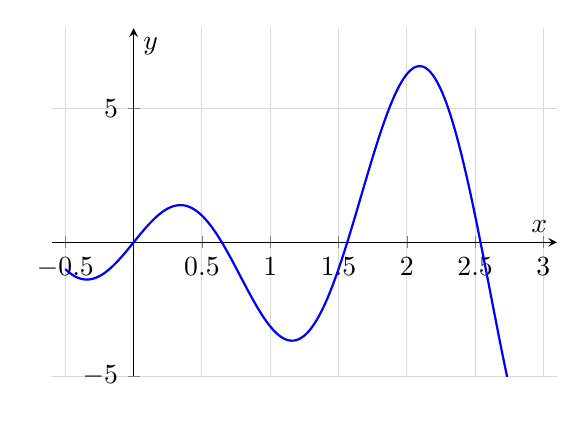
\begin{tikzpicture}
                \begin{axis}[
                    width=8cm,
                    height=6cm,
                    axis lines=middle,
                    xlabel=$x$,
                    ylabel=$y$,
                    xmin=-0.6,
                    xmax=3.1,
                    ymin=-5,
                    ymax=8,
                    grid=major,
                    grid style={gray!30},
                    samples=200,
                    domain=-0.5:3
                ]
                    \addplot[blue, thick] {pi*x*cos(pi*x*180/pi)+sin(pi*x*180/pi)};
                \end{axis}
            \end{tikzpicture}
        \end{image}
         \item Graph B:
        \begin{image}
            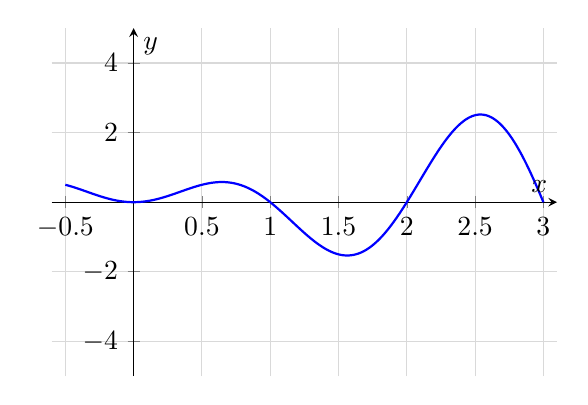
\begin{tikzpicture}
                \begin{axis}[
                    width=8cm,
                    height=6cm,
                    axis lines=middle,
                    xlabel=$x$,
                    ylabel=$y$,
                    xmin=-0.6,
                    xmax=3.1,
                    ymin=-5,
                    ymax=5,
                    grid=major,
                    grid style={gray!30},
                    samples=200,
                    domain=-0.5:3
                ]
                    \addplot[blue, thick] {x*sin(pi*x*180/pi)};
                \end{axis}
            \end{tikzpicture}
        \end{image}
         \item Graph C:
        \begin{image}
            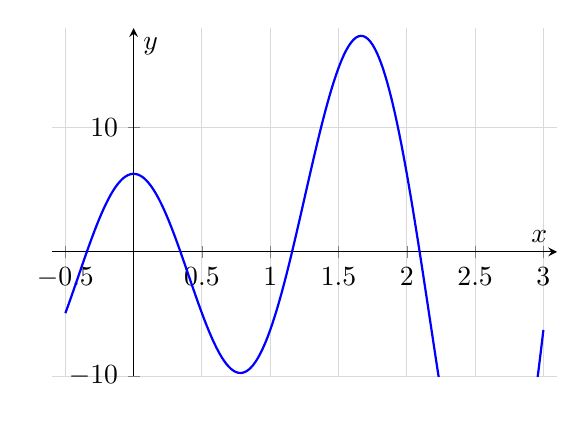
\begin{tikzpicture}
                \begin{axis}[
                    width=8cm,
                    height=6cm,
                    axis lines=middle,
                    xlabel=$x$,
                    ylabel=$y$,
                    xmin=-0.6,
                    xmax=3.1,
                    ymin=-10,
                    ymax=18,
                    grid=major,
                    grid style={gray!30},
                    samples=200,
                    domain=-0.5:3
                ]
                    \addplot[blue, thick] {-pi^2*x*sin(pi*x*180/pi)+2*pi*cos(pi*x*180/pi)};
                \end{axis}
            \end{tikzpicture}
        \end{image}
    \end{enumerate}

\end{exercise}


Problems adapted from Rogawski et al. \textit{Calculus: Early Transcendentals}, 4th Ed. 
\end{document}
